\documentclass[10pt]{article}
\usepackage{textcomp}
\usepackage{hyperref}
\usepackage{fullpage}
\usepackage{cite}
\usepackage{url}
\usepackage{footnote}
\usepackage{graphicx}
\usepackage{amsmath}
\usepackage{titlesec}
\usepackage[export]{adjustbox}
\usepackage{enumitem}
\usepackage{wrapfig}
\usepackage{bm}
\usepackage{appendix}
\usepackage[labelfont=bf]{caption}
\usepackage{subcaption}
\usepackage{lineno}

\setcounter{secnumdepth}{5} 

\setcounter{tocdepth}{5}

\renewcommand{\thetable}{S\arabic{table}}
\renewcommand{\thefigure}{S\arabic{figure}}
\renewcommand{\thesection}{S\arabic{section}}

\begin{document}

{\huge \textbf{Supporting Information to Naus et al. (2018)}}


\section{Procedure to obtain hemispheric-average MCF mixing ratios}
\label{sup:pseudo_obs}

To aggregate individual measurements of atmospheric air samples to a consistent record of hemispheric average mixing ratios requires correct interpretation of the information contained in the samples. For CH$_4$, CO$_2$ and in principle also for other gases, NOAA has developed \href{https://www.esrl.noaa.gov/gmd/ccgg/about/global_means.html}{a comprehensive interpolation algorithm} that approximates these averages. For example, the algorithm functions with gaps in the data and with a changing station network. For MCF, such an algorithm is not available. Instead, we applied an averaging scheme similar to \cite{montzka2011}. In this scheme, we first generated monthly means for each station that cover the whole time period of interest. Next, we aggregated the individual stations to hemispheric averages. 

Aggregating measurement data to monthly means requires several steps. Firstly, we linearly interpolated between measurements to obtain daily data. These daily averages were then straightforwardly averaged to monthly means. This worked reasonably well when each month has one or more measurements available. However, for most stations there were multi-month gaps. If more than one consecutive month was missing, we instead substituted values of nearby stations, corrected by an offset assumed to be constant through time. As an example, the offset between Cape Grim and South Pole is relatively constant, so if either station misses multiple months, a good approximation is obtained by substituting the other's values corrected for by the offset. This worked well when multiple stations that represent a similar air mass were available. The exception was the American Samoa Observatory (SMO), for which we only linearly interpolated in time. The implications of this exception were small, as the SMO record had few multi-month gaps in data coverage. Finally, to combine the monthly means of individual stations into hemispheric averages, we computed a weighted average. We combined sites that represent similar air masses in groups. A group's weight reflected the fraction of air mass that the group represented. Mostly, we used the cosine of the average latitude of the sites included in each group. Global mean mixing ratios that were derived using this procedure are shown in Figure~\ref{fig:ymix} (red line in the right panel).

A crucial question in this procedure is how to estimate uncertainties in derived averages. A common technique for estimating uncertainties is a bootstrapping procedure. used, for example, in \cite{turner2017}. In bootstrapping, different surface network realizations are randomly generated by counting some stations multiple times, while others are left out entirely. The spread in averages derived from the different network realizations then gives some measure for the uncertainties of these averages. For CH$_4$, this is how the uncertainties reported by NOAA (and used in this study) are derived. For MCF however, fewer stations are available, so that bootstrapping becomes less robust. Moreover, timeseries of annual means per station, as we derived them here, can be interdependent because of the substitution-technique described above. For these reasons, we adopted a different approach to derive uncertainties for MCF.

The procedure we adopted to derive uncertainties for MCF was based on the method presented by \cite{rigby2017}. In \cite{rigby2017}, the annual mean standard deviation (SD) of the MCF timeseries per surface site was used as a measure of the uncertainty in hemispheric means. We also used this measure, but we first removed an exponential trend from the timeseries at each station, before deriving the annual mean SD. This trend removal prevented the long-term trend in the MCF measurements from dominating the derived uncertainties. The SD in the residuals mainly resulted from source-sink variations, meteorological variability and measurement uncertainty. We deem this a more appropriate measure for uncertainty than the long-term trend. The trend removal reduced the annual mean SD per station from around 5\% (as in \cite{rigby2017}) to 1.5\%. 
Next, we used a Monte-Carlo simulation to propagate the uncertainty per station to an uncertainty in the global and hemispheric means. In the Monte-Carlo simulation, we perturbed the annual means per station proportional to the annual mean SD per station, and derived new global and hemispheric means. The SD of each quantity derived from the resulting ensemble was used as a measure for uncertainty. This Monte-Carlo approach accounts for the fact that stations are not expected to be influenced by the same variability at the same time, so that their errors should be largely uncorrelated. The time-dependent uncertainties in the global mean growth rate and in the rate of change of the IH gradient varied between 0.5$-$0.7\% and 1.0$-$1.5\% respectively. As can be expected from the modifications we have made to their method, this is significantly lower than the uncertainties adopted by \cite{rigby2017}, though still higher than the errors derived from the TM5 simulations (see Table 2). 

The timeseries of MCF we have derived, along with the corresponding uncertainties, are presented in a supplemental dataset, along with the same parameters for CH$_4$.

\section{The nudged simulation}
\label{sup:nudging}

In this supplement, we discuss the nudged simulation and some of its results. In the nudged simulation, we nudged the model to observations from NOAA surface sites, following a procedure analogous to \cite{banda2015}. In essence the nudging approach is a crude mass-balance inversion. We compared modelled mixing ratios at ground level at the dateline to latitudinally interpolated, monthly mean observations from the NOAA network, under the assumption that both of these are representative of the background atmosphere at that latitude. Then, we scaled the entire latitude band according to the model-to-observation ratio using a relaxation time of 100 days, to ensure that the model follows the long-term trend in real-world observations. Since the nudging does not depend on the a priori emission and loss fields, the nudged run provides a good test for the sensitivity of our conclusions to the source-sink distribution used.

\begin{figure}[t]
\centering
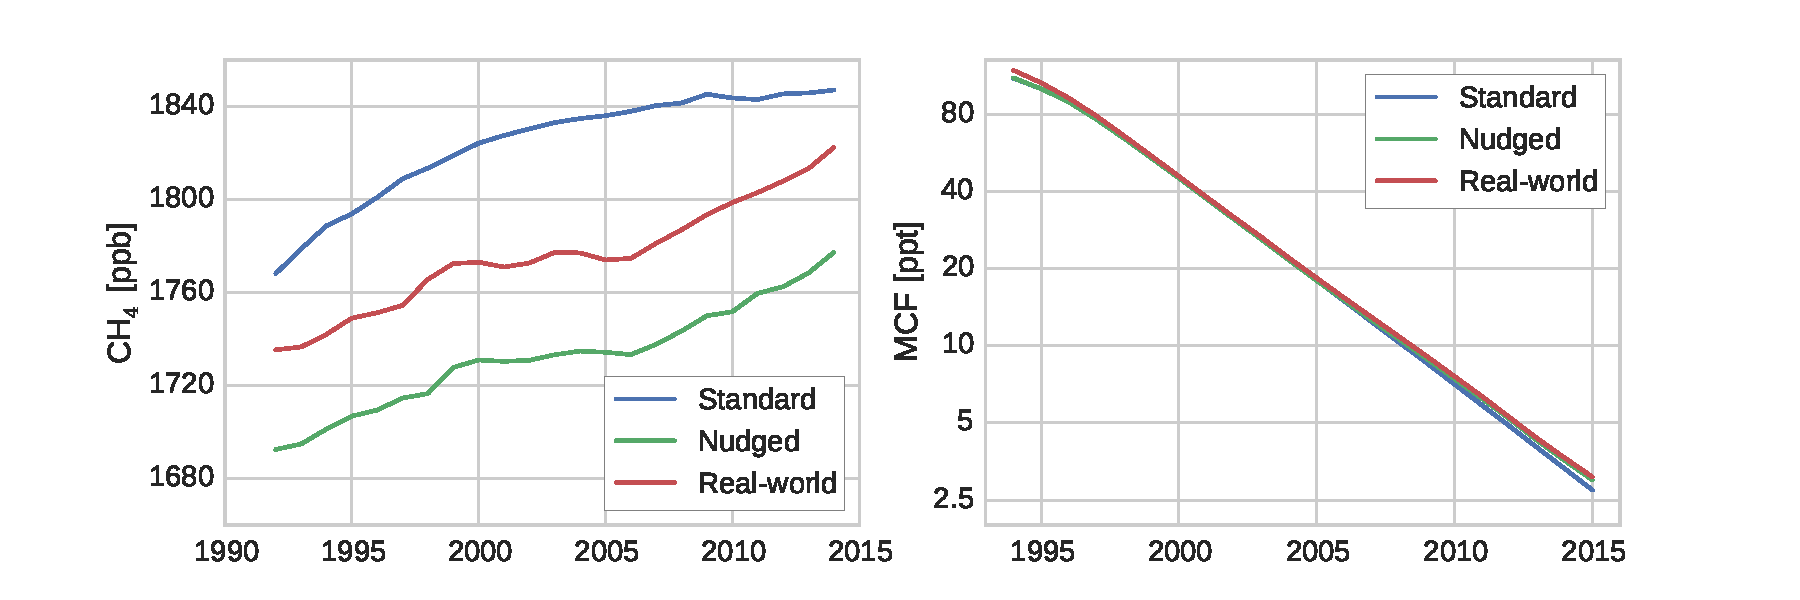
\includegraphics[width=12cm]{appendix/nudge_nonudge_obs_comparison.pdf}
\caption{Global, annual mean mixing ratios for CH$_4$ (left) and MCF (right) as derived from model-sampled observations from the standard and nudged simulation, and from real-world NOAA observations.}
\label{fig:ymix}
\end{figure}

Figure~\ref{fig:ymix} shows the global, annual mean mixing ratios of MCF and CH$_4$ as derived from model-sampled observations in the standard simulation and in the nudged simulation, and as derived from real-world NOAA data. For all three timeseries, the same averaging algorithms were used. The standard simulation for CH$_4$ performed poorly, as can be expected from a simulation with annually repeating emissions and constant loss fields. The nudged run captures the rough characteristics of CH$_4$ growth rate variations much better: the 2000-2006 stagnation and the renewed growth after 2007 are reproduced quite well.
For MCF, the standard run already captured the important aspects of the global atmospheric decline. However, from 2008 onwards the standard simulation increasingly underestimated MCF mixing ratios. Therefore, the nudged run tends to add MCF towards the end of the simulation. 

Observations sampled from the nudged run and real-world NOAA observations still differed for two reasons. Firstly, for the nudging, we did not compare mixing ratios at the site location, but at the dateline. Because we scaled the entire latitude band in the lower atmosphere, also the site location is nudged, but only indirectly. This difference is likely driving the systematic offset between annual means derived from the nudged runs and from the real-world annual means of CH$_4$ (left panel in Figure~\ref{fig:ymix}). At the dateline itself, the latitudinal fields used for nudging and the its modelled counterpart overlapped near perfectly. Secondly, only a subset of the measurement sites that were used for averaging, were used for nudging. We want to stress that the resulting differences are not important for our purposes, as our main objective was to test the sensitivity to a different, somewhat more realistic emission distribution, rather than provide a full inversion.

\begin{figure*}[t]
\centering
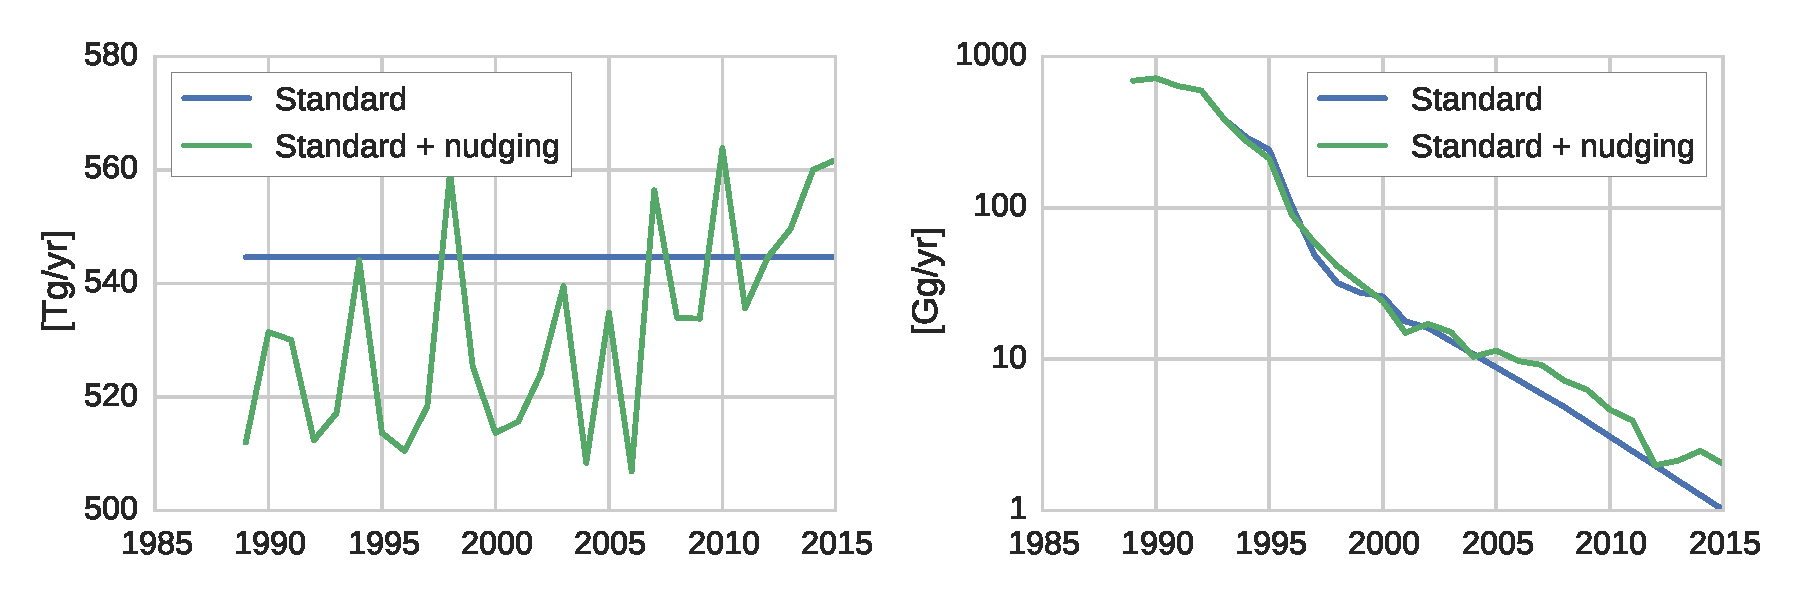
\includegraphics[width=12cm]{appendix/nudged_emissions.pdf}
\caption{Global, annual emissions of CH$_4$ (left) and MCF (right). Standard emissions are the emissions as used in all our TM5 simulations, while the standard+nudged emissions are the result of adding the global, annual mean nudging to the standard emissions.}
\label{fig:nudge_emi}
\end{figure*}

To give an impression of the nudging strength, Figure~\ref{fig:nudge_emi} shows the global emissions both from the standard and from the nudged TM5 simulation, if the derived nudging term (positive or negative) is assumed indicative of variations in emissions. Note that this interpretation is arbitrary, as nudging can also indicate variations in the loss fields. For CH$_4$, nudging can be quite extreme, with interannual variations of up to 40 Tg/yr. Though part of these emission variations may be real, the extreme extent of the variations likely resulted from overfitting or incorrect assignment of emissions to certain latitudes. This reveals the limitations of the nudging approach. For MCF, there was a clear need for additional emissions in later years with respect to our initial assumption that emissions declined with 20\%/year after 2006. Since differences in MCF mixing ratios between the standard run and real-world observations were especially high at Mace Head (not shown), this would indicate some ongoing European emissions.

\section{Interhemispheric asymmetries in correlations between k, OH and CH$_4$/MCF}
\label{sup:oh_ratio}

\subsection{Introduction}
In Section 3.1.3 it is outlined that the IH OH ratio to be used in a two-box model is not necessarily the same as the physical IH OH ratio. For example, in our 3D simulations runs, the IH ratio of the OH fields was 0.98, while the OH ratio seen by CH$_4$ was 1.05: a difference of 7\%. The differences are a result of first averaging k, OH, and CH$_4$/MCF per hemisphere, per year individually, and subsequently calculating the hemispheric loss (as in a box model), compared to a 3D model, where the loss is integrated over the cells that make up the hemisphere. Because of spatio-temporal correlations between the parameters involved (OH, k$_{OH}$, tracer distribution) and from hemispheric asymmetries in these correlations, differences between these two approaches arise. In this section, we outline in more detail which correlations predominantly drive the differences.

First, we define the ratio $r$ in equation \ref{eq:rcor}. The overline denotes the average over spatial and/or temporal dimensions. The ratio $r$ is unity for uncorrelated parameters,  and $r>1$ for positive and $r<1$ for negative correlations. The ratio $rr$ denotes the IH ratio of $r$ (Equation \ref{eq:rrcor}). If $rr>1$, the correlation is stronger in the NH than in the SH, and the reverse is the case for $rr<1$. Thus, while $r$ is a measure for the strength of the correlation in one hemisphere, $rr$ is a measure for the IH asymmetry in this correlation.

\begin{equation}
r[a, b, ...] = \frac{\overline{a \ b \ ...}} {\overline{a\vphantom{b}} \ \overline{b} \ \overline{...\vphantom{b}}}
\label{eq:rcor}
\end{equation} 

\begin{equation}
rr[a, b, ...] = \frac{r[a, b, ...]_{NH}}{r[a, b, ...]_{SH}}
\label{eq:rrcor}
\end{equation}

\begin{figure*}[t]
\centering
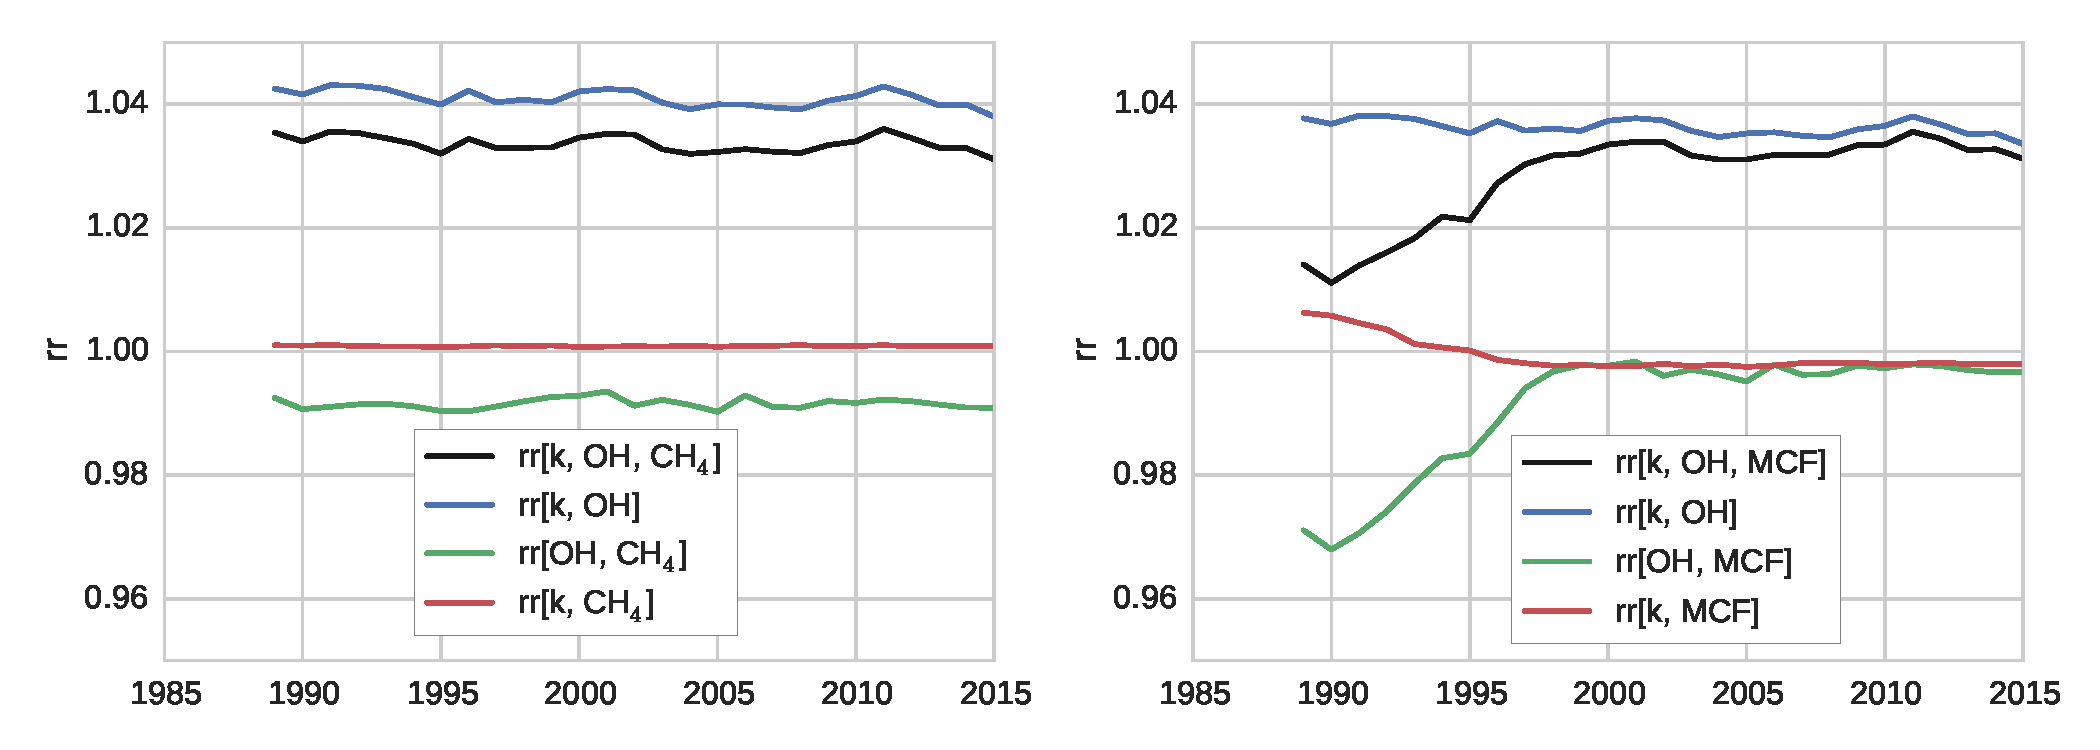
\includegraphics[width=12cm]{appendix/rr_full.pdf}
\caption{The annually averaged $rr$ ratios, as defined in Equation~\ref{eq:rrcor}, for the different components of chemical loss of CH$_4$ (left) and MCF (right).}
\label{fig:rr_full}
\end{figure*}

Ratios $rr[k, OH, CH_4]$ and $rr[k, OH, MCF]$ were both found to deviate significantly from 1 in the 3D simulations we used to tune our two-box model. This means that multiplying the hemispheric, annual averages of each parameter in a two-box model does not reproduce the loss rate calculated in the full 3D simulation. We emphasize that this result and the following analysis are specific to the OH field described in \cite{spivakovsky2000} and the implementation in TM5. There are three correlations that can drive the difference: between k$_{OH}$ and OH, between k$_{OH}$ and CH$_4$/MCF and between OH and CH$_4$/MCF. The contributions by each of these three to the asymmetry is shown in Figure~\ref{fig:rr_full}. From this figure, it can already be inferred that the main driver of both $rr[k_{OH}, OH, CH_4]$ and $rr[k_{OH}, OH, MCF]$ being greater than 1 is the correlation between k$_{OH}$ and OH, while the time-dependent behaviour of the IH OH ratio of MCF is driven predominantly by the correlation between OH and MCF. In the following, we discuss each of the three correlations in more detail.

\subsection{Correlation between reaction coefficient k$_{OH}$ and OH}

As the reaction coefficient k$_{OH}$ of both MCF and CH$_4$ are a direct function of only temperature (T), the spatial distribution of k$_{OH}$ and T are identical. For this reason, the correlation between k$_{OH+CH_4}$ and OH and k$_{OH+MCF}$ and OH are similar. Here, we discuss only k$_{OH+CH_4}$. OH and k$_{OH}$ are strongly positively correlated: spatially, with maxima in the tropics, and minima at the poles; and temporally, with maxima in the summer hemisphere and minima in the winter hemisphere. However, this correlation is stronger in the NH than in the SH, resulting in $rr[k_{OH}, OH]>1$ (blue lines in Figure \ref{fig:rr_full}; black line in Figure \ref{fig:koh_corr}). This effect turns out to be the main driver of both $rr[k_{OH}, OH, CH_4]$ and $rr[k_{OH}, OH, MCF]$ being greater than 1. The asymmetry is the integrated effect of correlations in the latitudinal, longitudinal, vertical and seasonal dimension. To assess the contribution of each dimension to the correlation asymmetry, we first averaged k$_{OH+CH_4}$ and OH over all but one dimension before computing $rr$. In this way, we isolate the influence of one dimension on the asymmetry. The result is shown in Figure \ref{fig:koh_corr}. 

\begin{figure}[t]
\centering
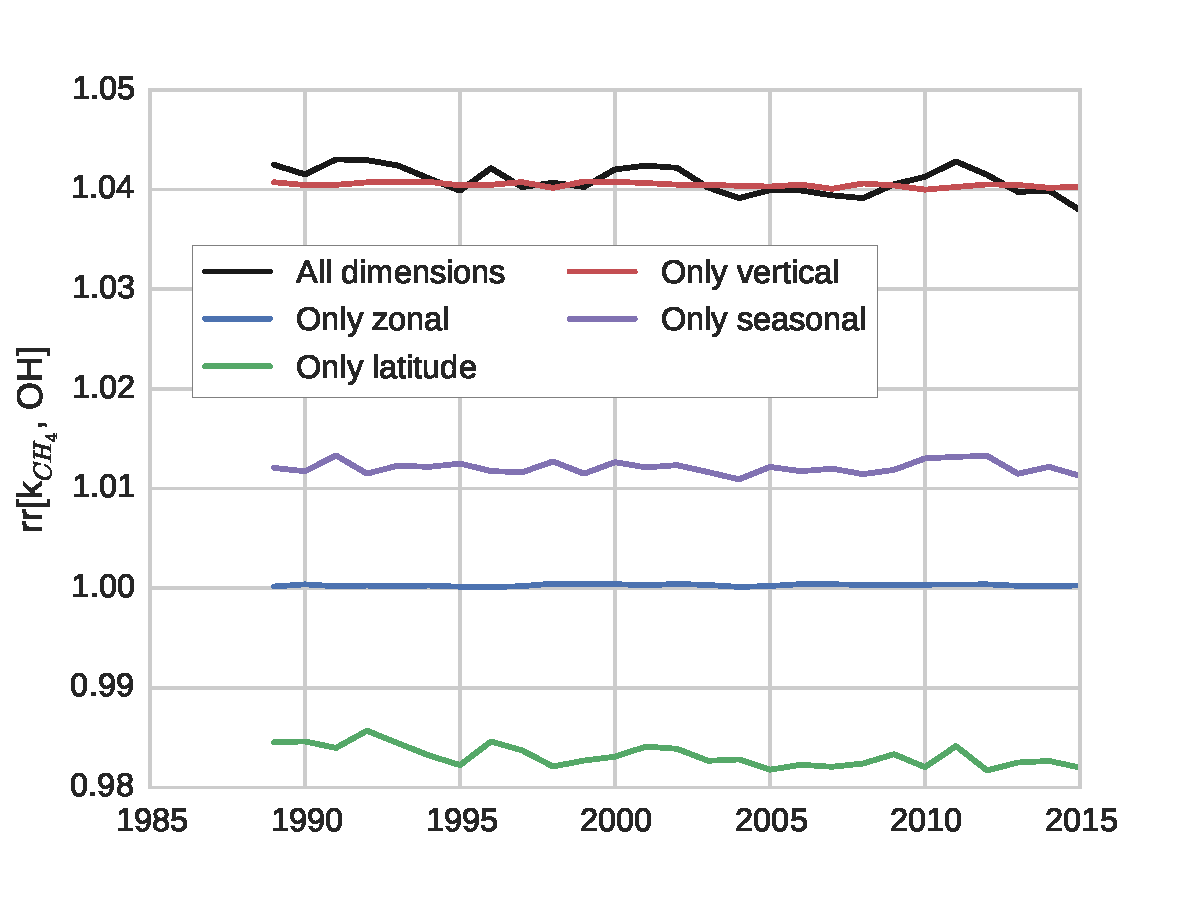
\includegraphics[width=8.3cm]{appendix/rr_koh.pdf}
\caption{The annually averaged evolution of the $rr[k_{CH_4}, OH]$ ratio, as defined in Equation~\ref{eq:rrcor}. The contribution from each dimension is isolated by only considering that dimension for the $rr$ ratio. Note that the black line corresponds to the blue line in the left panel of Figure~\ref{fig:rr_full} }
\label{fig:koh_corr}
\end{figure}

\begin{figure}[t]
\centering
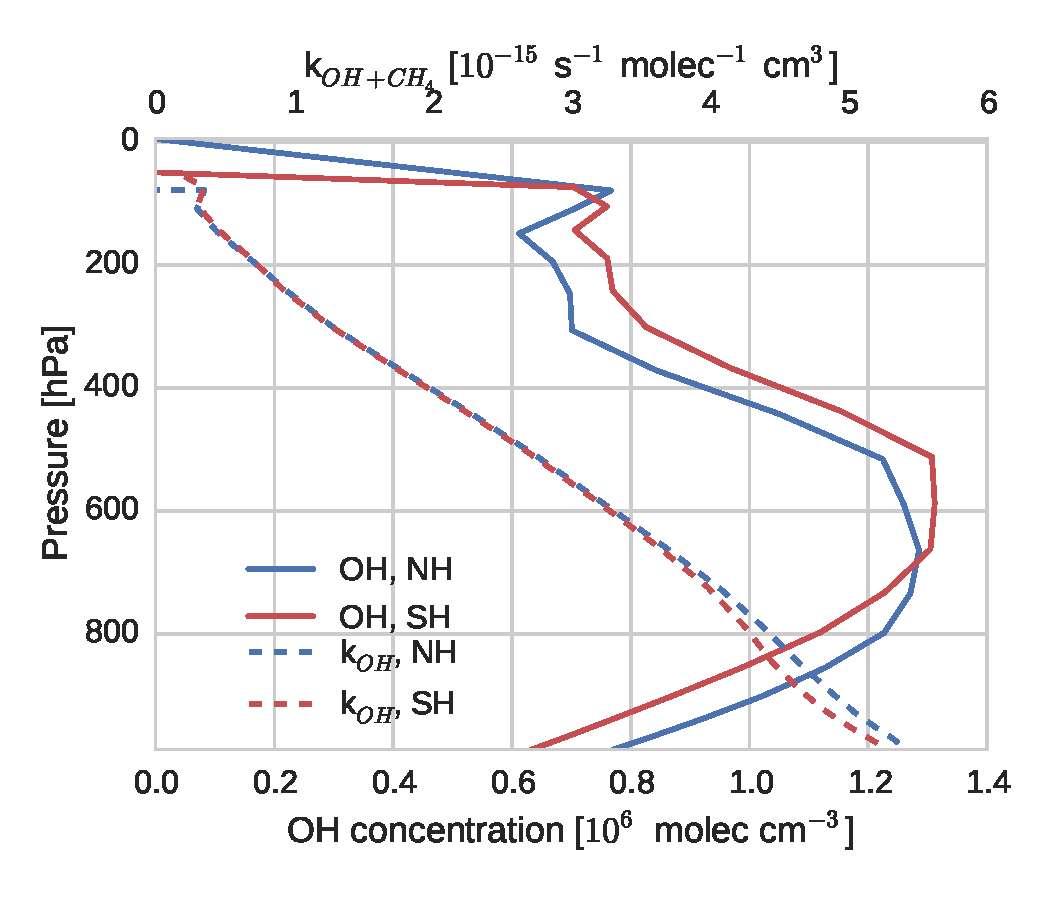
\includegraphics[width=8.3cm]{appendix/OH_vertical.pdf}
\caption{The average vertical distribution of tropospheric OH (solid lines, bottom y-axis) and k$_{OH+CH_4}$ (dashed lines, top y-axis) NH (blue) and in the SH (red).}
\label{fig:vert_oh}
\end{figure}

The largest effect is seen when isolating the vertical dimension, which gives an $rr$ close to the full $rr$ (red line in Figure \ref{fig:koh_corr}). Further analysis reveals that this is because the vertical distribution of OH in the NH and SH is different. More precisely, the maximum in OH is located at lower altitude in the NH than in the SH (Figure~\ref{fig:vert_oh}). This is likely driven by higher NO$_x$ emissions in the NH, which increases OH recycling close to the surface  (\cite{spivakovsky2000}). At lower altitudes temperatures are higher, and as a consequence the correlation between k$_{OH}$ and OH is strongest in the NH.

\begin{figure}[t]
\centering
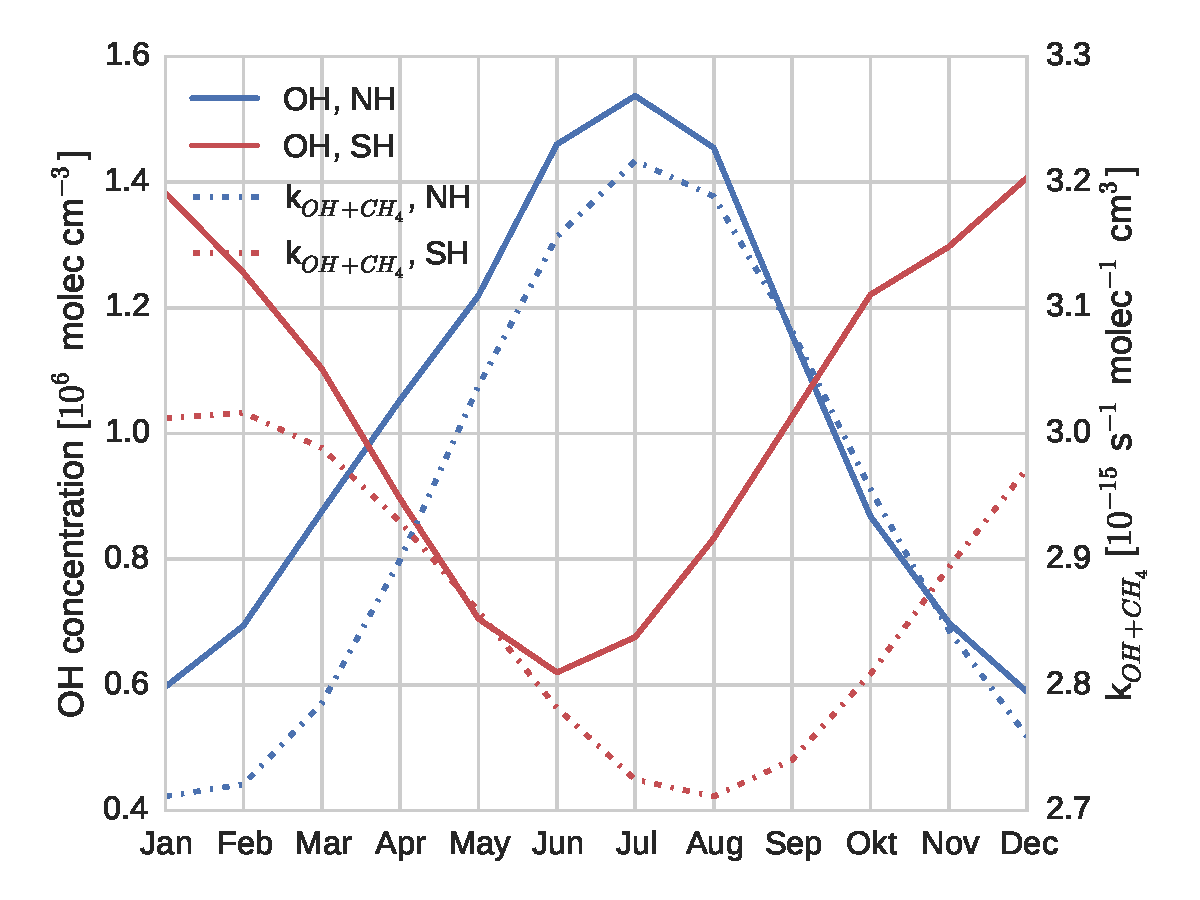
\includegraphics[width=8.3cm]{appendix/OH_seasonal.pdf}
\caption{The seasonal cycle of tropospheric OH (left axis, solid lines) and k$_{OH}$ (right axis, dashed lines) in the NH (blue) and in the SH (red).}
\label{fig:seas_oh}
\end{figure}

An effect in the same direction is seen for the seasonal component. Figure \ref{fig:seas_oh} shows the seasonal cycle of OH and k$_{OH+CH_4}$ in each hemisphere. In the NH, the two seasonal cycles are very well in line, while in the SH less so. Moreover, the seasonal cycle in temperature in the NH is stronger than in the SH. Both effects are likely a consequence of the higher land fraction in the NH, which results in a lower surface heat capacity. This drives a stronger and more direct response of temperature to seasonal variations in solar irradiance.

\begin{figure}[t]
\centering
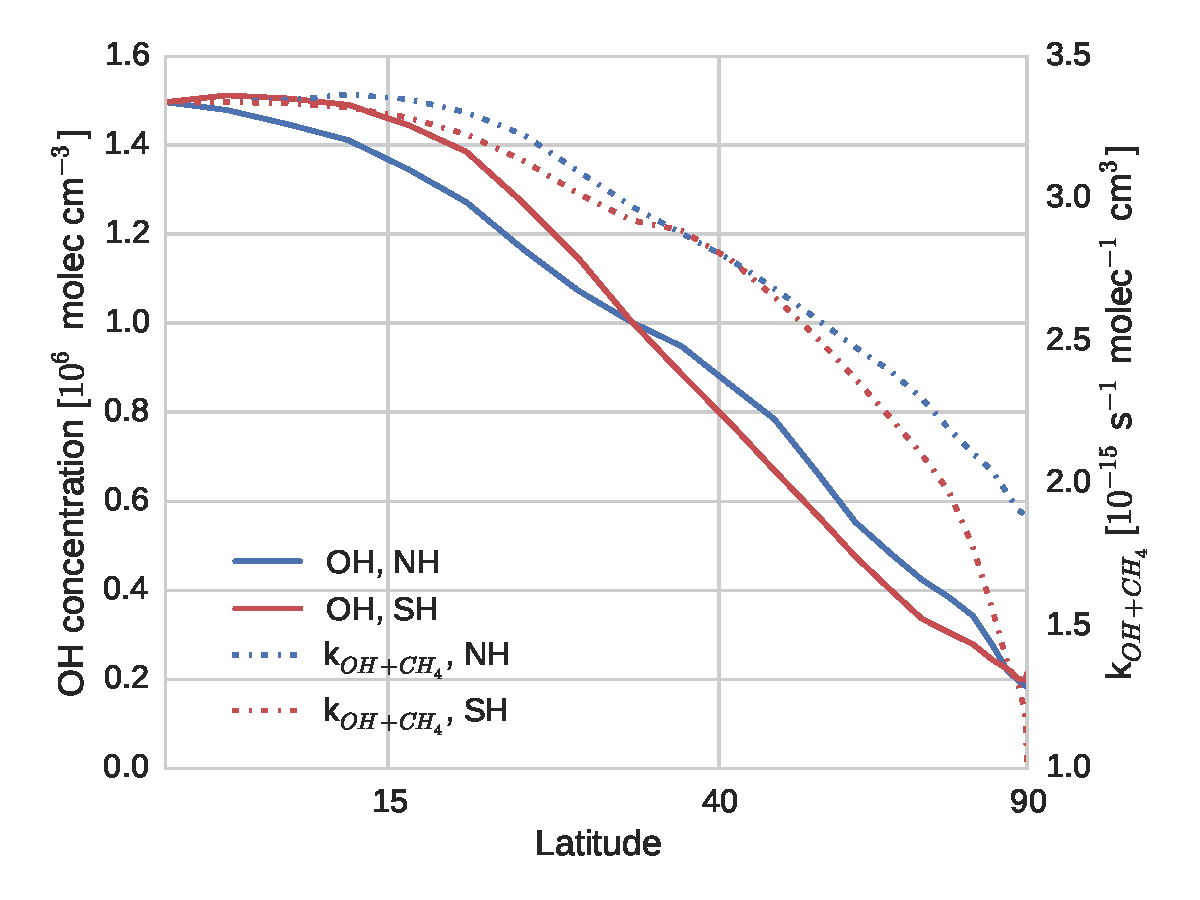
\includegraphics[width=8.3cm]{appendix/OH_latitude.pdf}
\caption{The latitudinal distribution of tropospheric OH (left axis, solid lines) and k$_{OH}$ (right axis, dashed lines) in the NH (blue) and in the SH (red).}
\label{fig:lat_oh}
\end{figure}

Finally, there is an opposing asymmetry in the latitudinal correlation. Figure~\ref{fig:lat_oh} shows that tropical OH is highest in the SH, whereas extra-tropical OH is highest in the NH. As temperatures are highest in the tropics, the correlation between temperature and OH is highest in the SH.

As expected, the dimension of longitude has only a small effect: both temperature and OH are relatively uniform zonally (not shown).

\subsection{Correlation between OH and CH$_4$/MCF}

\begin{figure}[t]
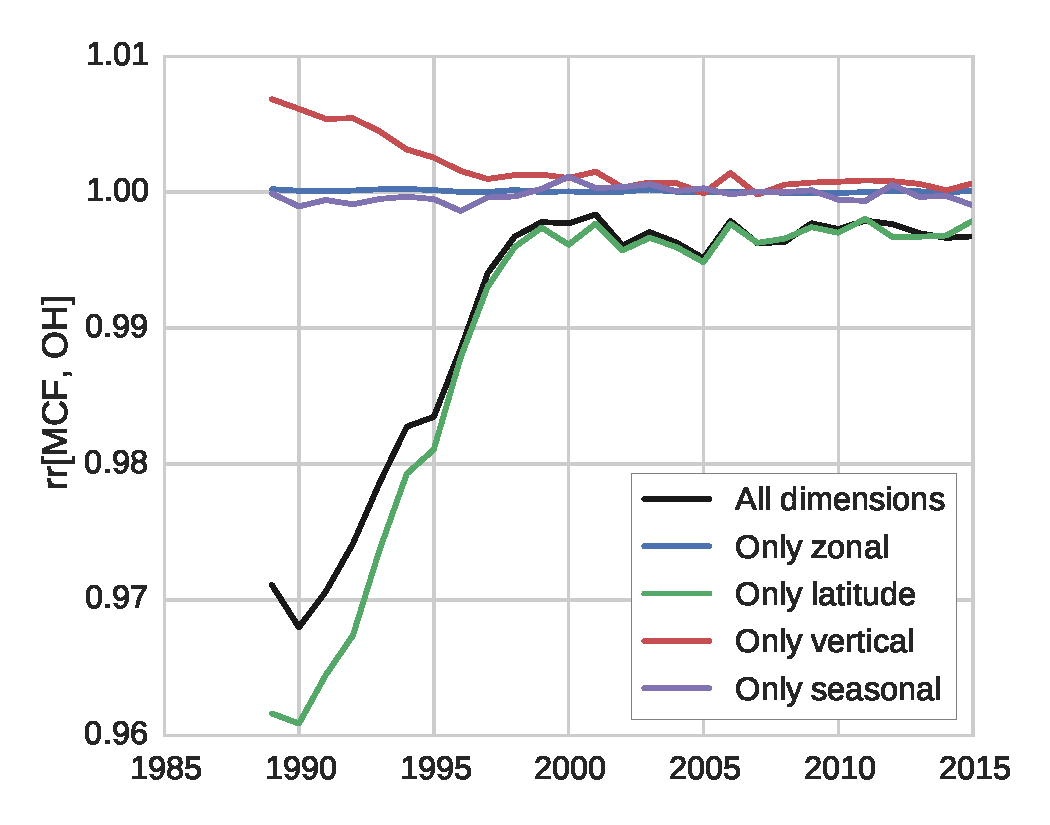
\includegraphics[width=8.3cm]{appendix/rr_oh_mcf.pdf}
\caption{The annually averaged evolution of the $rr[MCF, OH]$ ratio, as defined in Equation~\ref{eq:rrcor}. The contribution from each dimension is isolated by only considering that dimension for the $rr$ ratio. Note that the black line corresponds to the green line in the right panel of Figure~\ref{fig:rr_full}}
\label{fig:rr_ohmcf}
\end{figure}

Figure~\ref{fig:rr_full} shows that the trend in the IH OH ratio of MCF is largely driven by the $rr[OH,MCF]$ component of the correlation. It follows intuition that when the distribution of MCF strongly changes, then also the MCF distribution with respect to OH changes. Similar to $rr[k,OH]$, we can isolate the influence of each dimension on the asymmetry in the correlation (Figure~\ref{fig:rr_ohmcf}).

\begin{figure}[t]
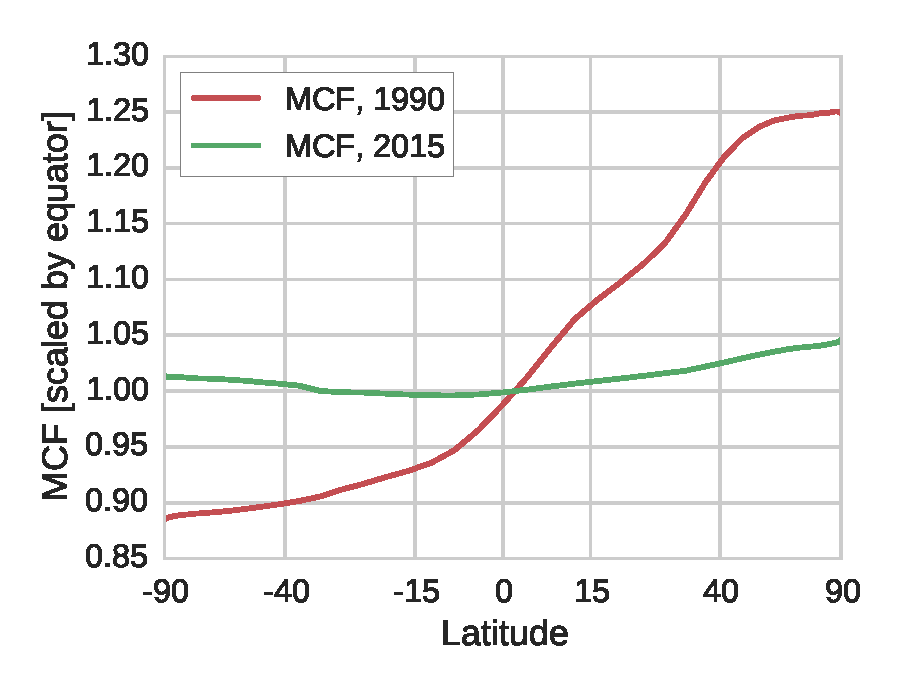
\includegraphics[width=8.3cm]{appendix/MCF_latitude_1990_2015.pdf} % first figure itself
\caption{The latitudinal distribution of MCF in 1990 and in 2015. MCF mixing ratios are scaled by MCF mixing ratios at the equator.}
\label{fig:mcf_lat}
\end{figure}
\begin{figure}[t]
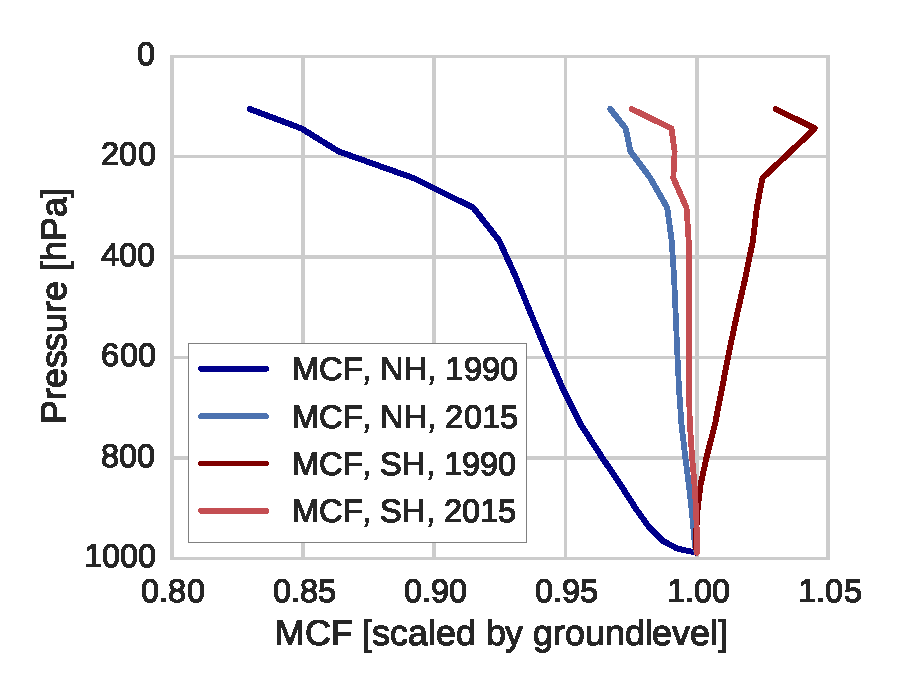
\includegraphics[width=8.3cm]{appendix/MCF_vertical_1990_2015.pdf} % second figure itself
\caption{The vertical distribution of MCF in 1990 and in 2015. MCF mixing ratios are scaled by ground-level MCF.}
\label{fig:mcf_vert}
\end{figure}

The largest contribution to $rr[OH,MCF]$ comes from the latitudinal component (green line in Figure \ref{fig:rr_ohmcf}). This is driven by the decreasing IH MCF gradient through time (Figure~\ref{fig:mcf_lat}). Initially, MCF decreases towards the tropics in the NH, and increases towards the tropics in the SH. As OH is highest in the tropics, MCF and OH are negatively correlated in the NH and positively correlated in the SH. This drives $rr[OH,MCF]<1$. The IH gradient largely disappears over time, so that $rr[OH,MCF]$ approaches 1. 

A weaker, opposite effect is seen in the vertical. Initially, NH MCF decreases with altitude strongly, while SH MCF slightly increases with altitude (Figure~\ref{fig:mcf_vert}). As OH maximizes at low altitude, this drives a positive correlation in the NH, compared to the weak negative correlation in the SH. This results in an $rr[OH,MCF]>1$. As the gradients disappear over time, so too does the asymmetric correlation. 

For CH$_4$, spatio-temporal gradients are smaller. However, it too has an $rr[OH,CH_4]<1$, mostly due to the IH gradient in CH$_4$.

\subsection{Correlation between reaction coefficient k$_{OH}$ and CH$_4$/MCF}

As indicated earlier, correlations between $k$ and OH are very high, and thus the correlation between k$_{OH}$ and CH$_4$/MCF behaves largely similar to the correlation between OH and CH$_4$/MCF. However, interestingly, the net effect on $rr$ can be opposite. In the early 90s, we find a positive trend in $rr[OH,MCF]$, while the trend in $rr[k_{OH+MCF},MCF]$ is negative (right panel in Figure~\ref{fig:rr_full}). This is because temperature, and thus $k$, have stronger and more unidirectional gradients in the vertical, compared to OH. Therefore, the correlation between mixing ratios and $k$ is dominated by the vertical dimension, whereas the correlation between OH and mixing ratios is dominated by the latitudinal dimension. This detail reveals the intricacies of the compensating effects in the final $rr$ ratio, and thus of the resulting IH OH ratio seen by different tracers.

\subsection{Conclusions on the IH OH ratio}

In conclusion, the symmetry between the NH and the SH that is implicitly assumed in the typical two-box set-up does not necessarily hold. This means that different tracers potentially require different IH OH ratios. That different tracers might be exposed to different atmospheric oxidative capacities has been noted before \cite{lawrence2001}. However, we quantify exactly the contributions of different parameters and dimensions on the ratio. The most important implication of this analysis is the sheer number of parameters that the final OH ratio hinges on (e.g. IH gradient; vertical profile; temperature dependence of $k_{OH}$). This makes it very difficult to predict how the ratio would vary under changing conditions and for different tracers. Of course, our results depend strongly on the specific OH distribution and 3D transport model that is used, but the OH distribution and 3D model we use has been shown to result in realistic CH$_4$ mixing ratio fields (\cite{patra2011}; \cite{huijnen2010}). Moreover, the observation that such large deviations between tracers and in time are possible, will likely hold for any OH distribution and 3D transport model.

\section{Robustness of derived interhemispheric exchange rates}

In Section 3.1.1, we present IH exchange rates ($k_{IH}$) for CH$_4$, MCF and SF$_6$ as derived from a TM5 simulation. Here, we explore the robustness of the derived IH exchange rates in three scenarios. Firstly, we repeated the standard simulation, but with annually repeating meteorological fields (hereafter referred to as the RM simulation). We repeated meteorological fields from the year 2012, but results were qualitatively similar if a different year was chosen. Secondly, we redid the TM5 to two-box parametrization (see Section 2.2.2), but with the two hemispheres demarcated at 8$^{o}$N instead of at the equator, which is more representative of the average position of the inter-tropical convergence zone (ITCZ). Thirdly, we investigated the exchange rate in the nudged simulation (Supplement~\ref{sup:nudging}), which gives a measure for the sensitivity of derived rates to realistic variations in the source-sink distributions. The results are shown in Figure~\ref{fig:kih}.

\begin{figure}[t]
\centering
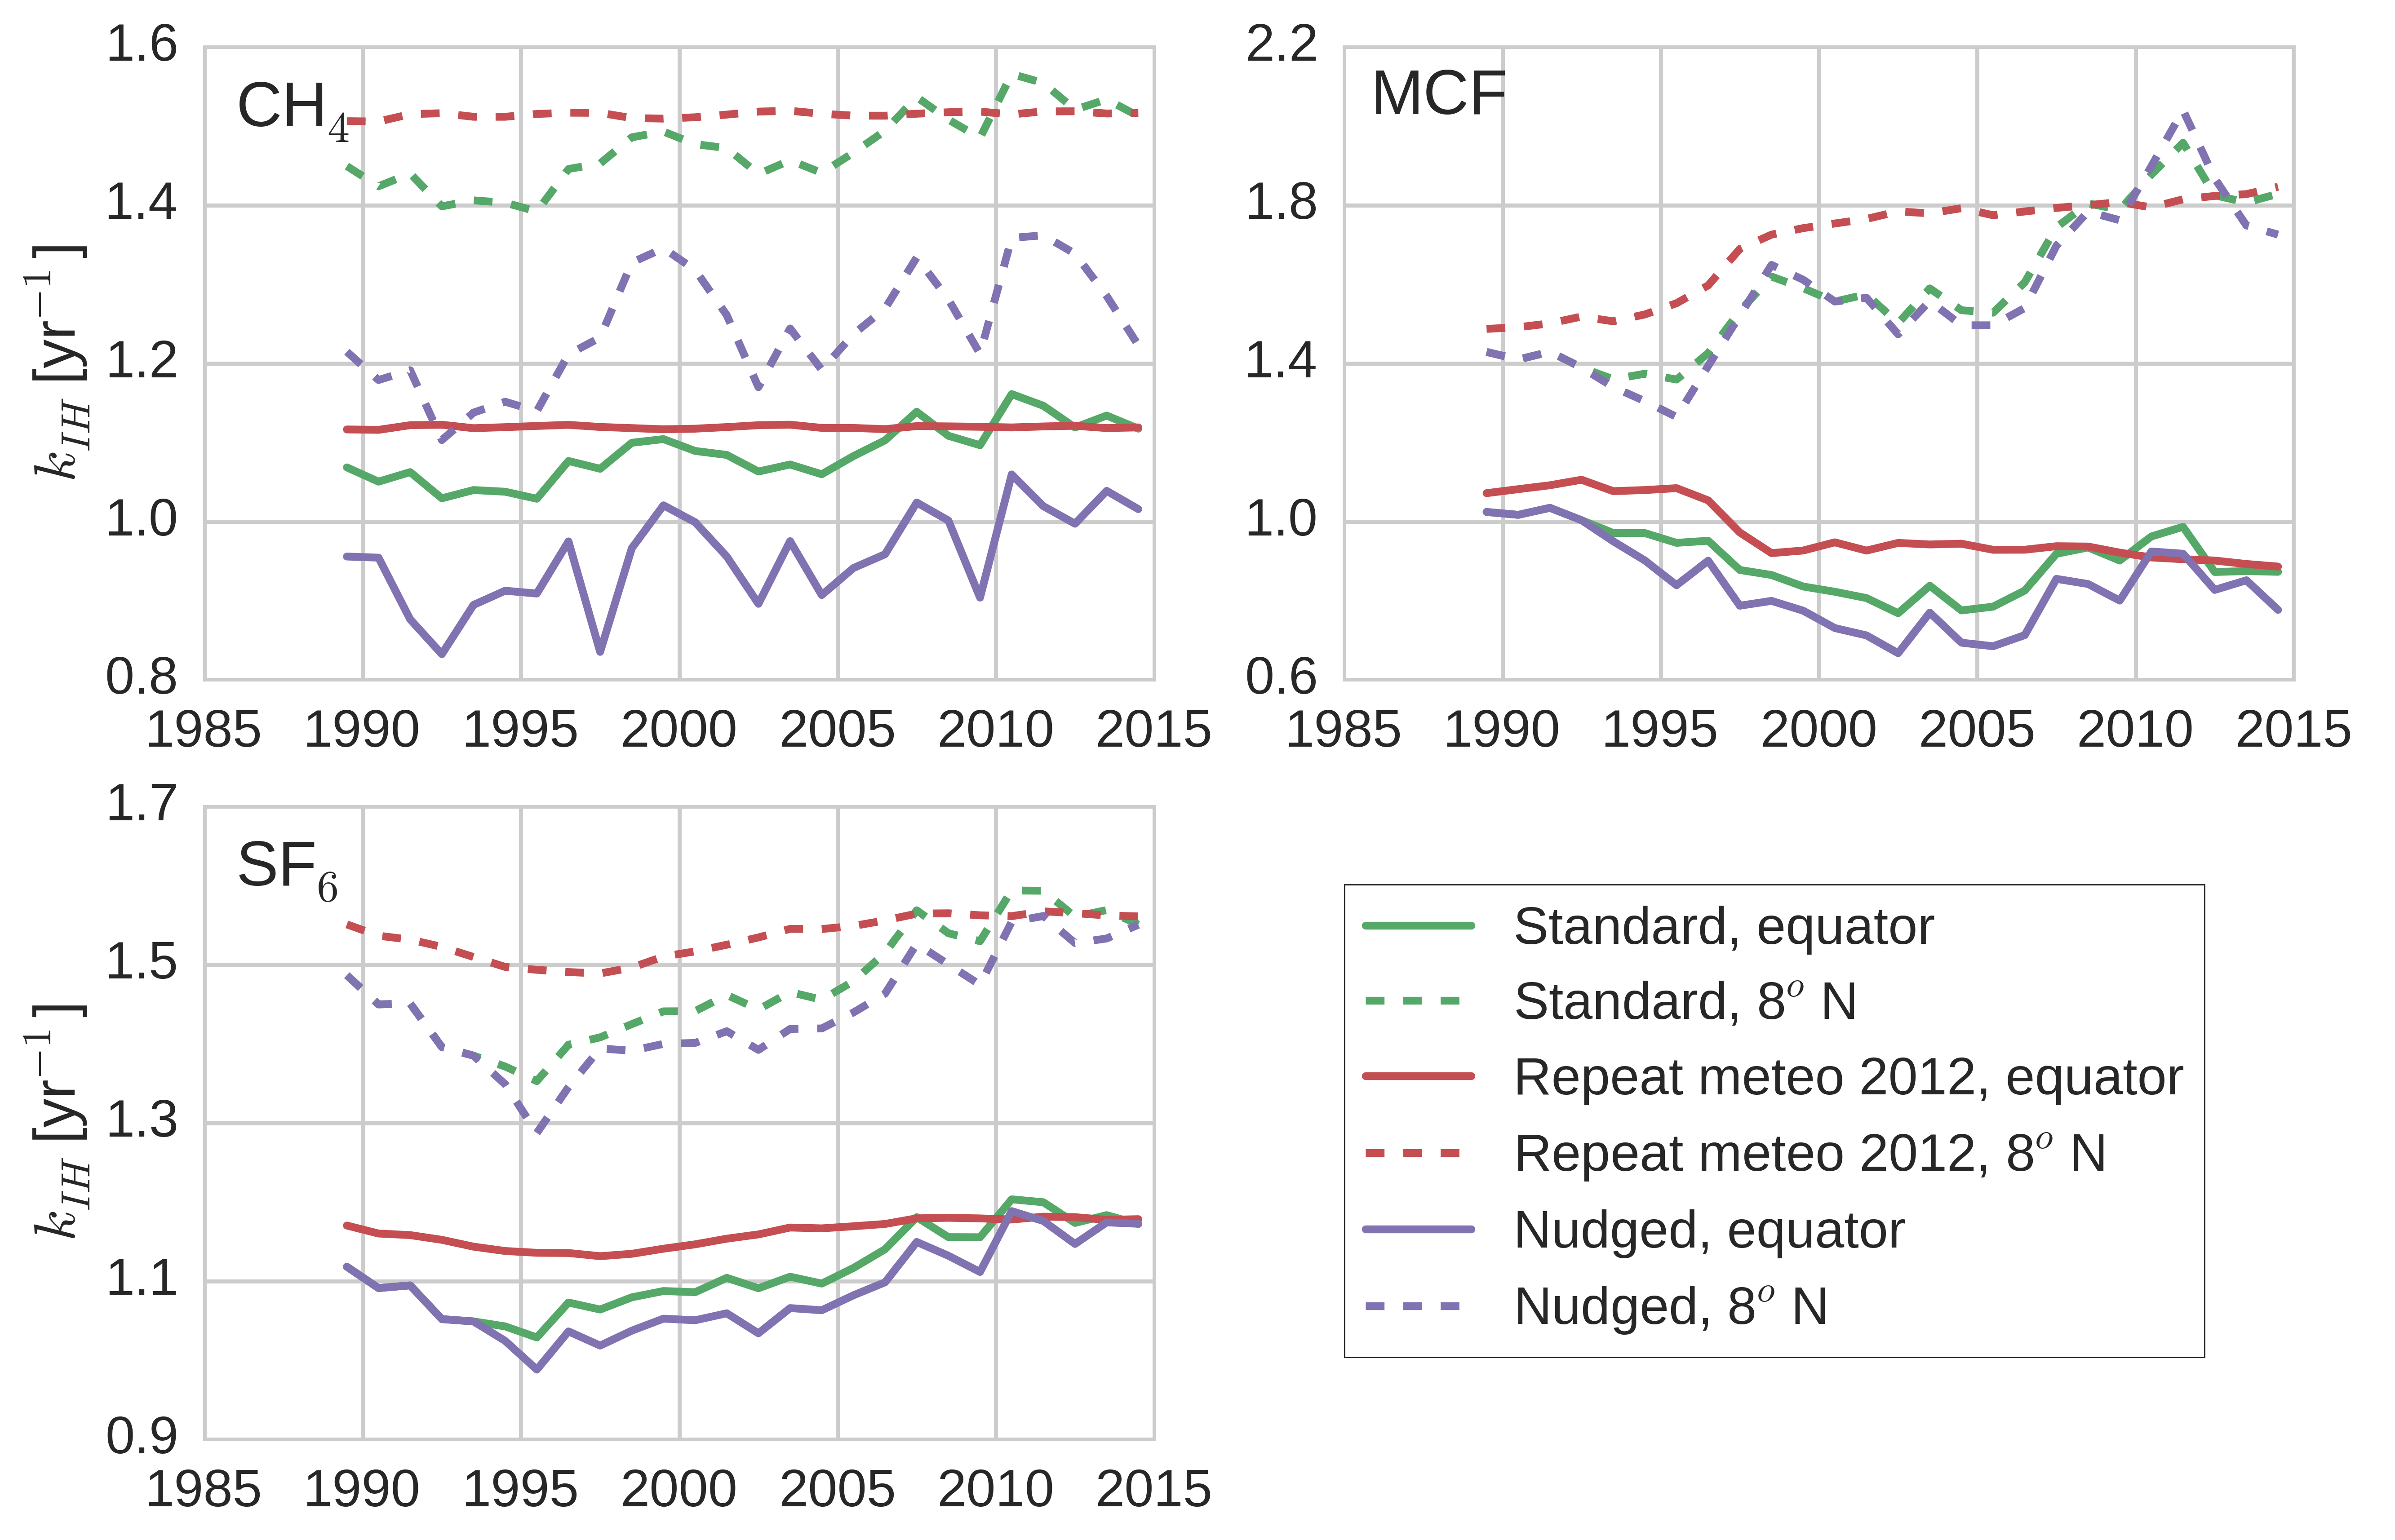
\includegraphics[width=12cm]{appendix/kih_all_comp.png}
\caption{The IH exchange coefficients for CH$_4$ (top left), MCF (top right) and SF$_6$ (bottom left) as derived from a set of sensitivity tests. Rates derived from the standard simulation (green), a simulation with annually repeating meteorology (red) and the nudged simulation (purple) are shown. Additionally, for each of the three simulations, we show the sensitivity of the IH exchange rate to the hemispheric demarcation in the derivation, by shifting it from the equator (solid lines) to 8$^{o}$N (dashed lines). Note that the range on the axes differ for the three tracers.}
\label{fig:kih}
\end{figure}

In the RM simulation, we isolated the influence of source-sink variations on the exchange rate. Since we used annually repeating source and sink fields for CH$_4$, the derived exchange rate showed nearly no variability in the RM simulation. This shows that all interannual variability and the trend we found in the standard simulation for CH$_4$ were driven by transport, and not, for example, by any spin-up effects.
For MCF and SF$_6$, interannual variations in the emission fields were implemented, and this was reflected in the IH exchange rate derived from the RM simulation. For SF$_6$, the emissions variations were small and gradual, and so were the variations in the IH exchange rate. For MCF, we found a decrease in IH exchange of 25\%, that coincided with the drop in MCF emissions. In the standard simulation this decrease was masked by transport variability, so that the exchange rate minimized in 2000-2005 and then recovered. This indicates that the derived IH exchange rate of MCF is especially sensitive to interannual variations in transport.

Next, we tested the influence of the position of the hemispheric demarcation on the IH exchange rate. For all three tracers, moving the division to 8$^{o}$N resulted in faster exchange rates. For CH$_4$ and for SF$_6$ the offset was nearly constant through time at 35\% and 33\% respectively. Thus, variability in the exchange rate was found to be robust with respect to the choice of hemispheric demarcation. For MCF, this was not the case. In fact, in the simulation with annually repeating meteorology, the decrease in IH exchange became an increase instead.
The choice of hemispheric demarcation is somewhat arbitrary, since there is not one meteorological dividing line which sharply isolates the two hemispheres. Yet the IH exchange variations of MCF were highly sensitive to the demarcation. The result is not so surprising, when considering that the IH exchange rate for MCF became ill-defined post-1998. After 1998, the latitudinal MCF mixing ratio gradient started to show a minimum in the tropics, where most exchange takes place, so that the net IH gradient is not well representative of the gradient against which transport takes place. Thus, if the IH gradient of MCF, as derived from surface networks, is to be used to disentangle OH from emissions, then a method needs to be found that correctly accounts for (variations in) the IH exchange.

Finally, the sensitivity to source-sink variations was quantified in the nudged simulation. We found that all tracers were somewhat sensitive to nudging, but that the overall tendencies were conserved. CH$_4$ was most sensitive, which can be expected, as it was nudged most strongly due to a poor fit to surface observations in the standard simulation. Most notably, we found a systematic shift to slower exchange rates for CH$_4$ in the nudged simulation. However, in general, years with positive anomalies in the standard simulation still have positive anomalies in the nudged simulation, albeit with a higher amplitude. Additionally, the positive trend for CH$_4$ and SF$_6$ persists, as does the minimum for MCF, even if it is slightly modified. Therefore, we conclude that the interannual variability of the derived IH exchange rates is quite robust with respect to source-sink variations of realistic magnitude.

In conclusion, we found that the IH exchange rates presented in Section 3.1.1 can be sensitive to prior assumptions in the 3D transport model, such as the source-sink distribution and the hemispheric demarcation. Especially for MCF we found a high sensitivity to hemispheric demarcation, which indicates that defining a two-box exchange rate for MCF is difficult. Moreover, we found that IH exchange of MCF was especially sensitive to transport variations. For CH$_4$ and SF$_6$, interannual source-sink variations were not as extreme, which resulted in a small sensitivity of their IH exchange rates to prior assumptions. Thus, the parametrization is in principle robust, unless a tracer's global distribution changed considerably.

%\nocite{*}
\bibliography{mybib}
%\bibliographystyle{copernicus}
\bibliographystyle{unsrt}

\end{document}